% This is sigproc-sp.tex -FILE FOR V2.6SP OF ACM_PROC_ARTICLE-SP.CLS
% OCTOBER 2002
%
% It is an example file showing how to use the 'acm_proc_article-sp.cls' V2.6SP
% LaTeX2e document class file for Conference Proceedings submissions.
% ----------------------------------------------------------------------------------------------------------------
% This .tex file (and associated .cls V2.6SP) *DOES NOT* produce:
%       1) The Permission Statement
%       2) The Conference (location) Info information
%       3) The Copyright Line with ACM data
%       4) Page numbering
%
%  However, both the CopyrightYear (default to 2002) and the ACM Copyright Data
% (default to X-XXXXX-XX-X/XX/XX) can still be over-ridden by whatever the author
% inserts into the source .tex file.
% e.g.
% \CopyrightYear{2003} will cause 2003 to appear in the copyright line.
% \crdata{0-12345-67-8/90/12} will cause 0-12345-67-8/90/12 to appear in the copyright line.
%
% ---------------------------------------------------------------------------------------------------------------
% It is an example which *does* use the .bib file (from which the .bbl file
% is produced).
% REMEMBER HOWEVER: After having produced the .bbl file,
% and prior to final submission,
% you need to 'insert'  your .bbl file into your source .tex file so as to provide
% ONE 'self-contained' source file.
%
% Questions regarding SIGS should be sent to
% Adrienne Griscti ---> griscti@acm.org
%
% Questions/suggestions regarding the guidelines, .tex and .cls files, etc. to
% Gerald Murray ---> murray@acm.org
%
% For tracking purposes - this is V2.6SP - OCTOBER 2002

\documentclass{acm_proc_article-csis8101}
\usepackage{color}

\newdef{definition}{Definition}
\newdef{example}{Example}

\begin{document}
%
% --- Author Metadata here ---
\conferenceinfo{COMP 9102 Surveys}{2017, CS Dept, HKU}
%\setpagenumber{50}
%\CopyrightYear{2002} % Allows default copyright year (2002) to be over-ridden - IF NEED BE.
%\crdata{0-12345-67-8/90/01}  % Allows default copyright data (X-XXXXX-XX-X/XX/XX) to be over-ridden.
% --- End of Author Metadata ---

\title{A Survey of Entity Similarity Measures on Heterogeneous Information Network}
%
% You need the command \numberofauthors to handle the "boxing"
% and alignment of the authors under the title, and to add
% a section for authors number 4 through n.

\author{
ZHU Zichen\\
Department of Computer Science\\
University of Hong Kong\\
Pokfulam Road, Hong Kong\\
\texttt{zczhu2@cs.hku.hk}
\and MA Chenhao\\
Department of Computer Science\\
University of Hong Kong \\
Pokfulam Road, Hong Kong \\
\texttt{chma2@cs.hku.hk}
}

\numberofauthors{2}
%
\maketitle
\begin{abstract}
According to recent studies, {\em heterogeneous information networks (HINs)} consisting of multiple types of entities and relations has shown its power in many disciplines, such as, computer science, social science, physics and so on. More and more researchers have noticed the importance of HIN analysis and many novel data mining tasks have been exploited in such networks, such as similarity search, clustering, and classification. Among those tasks, similarity measure on HINs, which is mainly to evaluate the similarity of entities, is the basis of many data mining tasks, such as clustering and classification. In this paper, we provide a survey of similarity measures on heterogeneous information networks. We will introduce basic concepts of heterogeneous information networks analysis, examine the recent developments on similarity measures and make a general evaluation of those similarity metrics.
% This paper provides a sample of a \LaTeX\ document which conforms to
% the formatting guidelines for ACM SIG Proceedings.
% It complements the document \textit{Author's Guide to Preparing
% ACM SIG Proceedings Using \LaTeX$2_\epsilon$\ and Bib\TeX}. This
% source file has been written with the intention of being
% compiled under \LaTeX$2_\epsilon$\ and BibTeX.

% The developers have tried to include every imaginable sort
% of ``bells and whistles", such as a subtitle, footnotes on
% title, subtitle and authors, as well as in the text, and
% every optional component (e.g. Acknowledgments, Additional
% Authors, Appendices), not to mention examples of
% equations, theorems, tables and figures.

% To make best use of this sample document, run it through \LaTeX\
% and BibTeX, and compare this source code with the printed
% output produced by the dvi file.
\end{abstract}


\section{Introduction}
Recently, researchers use heterogeneous information networks (HINs) to model real world relationships in many applications, especially for real systems containing multi-typed interacting components. For instance, in bibliographic database, like DBLP\footnote{http://dblp.uni-trier.de} \cite{sun2013mining}, papers are connected together via authors, venues and terms; and in Instagram\footnote{http://instagram.com}, photos or videos are linked together via users, locations, hashtags and comments. Compared to widely-used homogeneous information networks \cite{leroy2010cold, lichtenwalter2010new}, which are extracted from real interacting systems by simply ignoring the heterogeneity of objects and links or only considering one type of relations among one type of objects, the heterogeneous information network can effectively fuse more information and contain rich and specific semantics in nodes and links \cite{shi2017survey}.

Because of HIN's property of rich semantics and information, since the concept of heterogeneous information network and meta path proposed in 2009 \cite{sun2009rankclus} and 2011 \cite{sun2011pathsim}, respectively, more and more researchers have noticed the importance of heterogeneouse information network analysis and many novel data mining tasks have been developed in such networks, such as similarity search \cite{shi2012relevance,sun2011pathsim}, clustering \cite{sun2013pathselclus}. In other words, HIN analysis has become a hot topic rapidly in the fields of data mining, database and information retrieval, involving similarity measure, clustering, classification, link prediction, ranking, recommendation and information fusion on HINs \cite{shi2017survey}.

Among those analysis tasks, similarity measure is the fundamental problem of network analysis, because most high level tasks, such as clustering and classification, need to evaluate the similarity of objects or relations. What's more, most of the state-of-the-art homogeneous network similarity methods, which generally assume the networks don't carry semantics, do not generalize well in HINs, due to HINs' rich semantics. Thus, some similarity metrics based on meta-path, which represents semantics in HINs, have been designed to evaluate the similarity between entities or relations in HINs, such as PathSim \cite{sun2011pathsim} and RelSim \cite{wang2016relsim}. {\color{red} Maybe some figure of HIN and an example...}

In this paper, we attempts to clearly introduce basic concepts in heterogeneous network analysis and make a conprehensive investigation on contemporary research developments of similarity metrics on HINs. Then, we tentatively provide a general evaluation over some of these state-of-the-art algorithms to give some reference on similarity measure choosing in high level network analysis tasks, such as clustering and classification.

The following part is organized as follows. Section 2 introduces the basic concepts and examples about HIN. Section 3 presents recent designed similarity measures on HIN. Experiments and evaluation are conducted in Section 4. Finally, Section 5 summarizes and concludes this paper.

% The \textit{proceedings} are the records of a conference.
% ACM seeks to give these conference by-products a uniform,
% high-quality appearance.  To do this, ACM has some rigid
% requirements for the format of the proceedings documents: there
% is a specified format (balanced  double columns), a specified
% set of fonts (Arial or Helvetica and Times Roman) in
% certain specified sizes (for instance, 9 point for body copy),
% a specified live area (18 $\times$ 23.5 cm [7" $\times$ 9.25"]) centered on
% the page, specified size of margins (2.54cm [1"] top and
% bottom and 1.9cm [.75"] left and right; specified column width
% (8.45cm [3.33"]) and gutter size (.083cm [.33"]).

% The good news is, with only a handful of manual
% settings\footnote{Two of these, the {\texttt{\char'134 numberofauthors}}
% and {\texttt{\char'134 alignauthor}} commands, you have
% already used; another, {\texttt{\char'134 balancecolumns}}, will
% be used in your very last run of \LaTeX\ to ensure
% balanced column heights on the last page.}, the \LaTeX\ document
% class file handles all of this for you.

% The remainder of this document is concerned with showing, in
% the context of an ``actual'' document, the \LaTeX\ commands
% specifically available for denoting the structure of a
% proceedings paper, rather than with giving rigorous descriptions
% or explanations of such commands.

\section{Basic Concepts and Definitions}

In this section, we introduce some basic concepts about HIN and give some HIN examples. We first define the information network and heterogeneous information network.

An information network represents an abstraction of the real world, focusing on the entities and the relations among these entities.

\begin{definition}
{\bf Information Network} \cite{sun2013mining,sun2009ranking}. An information network is defined as a directed graph $G=(V,E)$ with an entity type mapping function $\varphi: V \rightarrow \mathcal{A}$ and a relation type mapping function $\psi: E \rightarrow \mathcal{R}$. Each entity $v \in V$ belongs to one particular entity type in the entity type set $\mathcal{A}: \varphi(v) \in \mathcal{A}$, and each relation $e \in E$ belongs to a particular relation type in the relation type set $\mathcal{R}: \psi(e) \in \mathcal{R}$. If two relations belongs to the same relation type, the two links share the same starting entity type as well as the ending entity type.
\end{definition}

Based on the definition of information network, we derive the definitions of heterogeneous/homogeneous information network.

\begin{definition}
{\bf Heterogeneous/homogeneous information network}. The information network is called heterogeneous information network if the type of entities $|\mathcal{A}|>1$ or the types of relations $|\mathcal{R}|>1$; otherwise, it is a homogeneous information network.
\end{definition}

For better understanding the entity types and relation types in a complex heterogeneous information network, the network schema provides a high-level description of a given heterogeneous information network.

\begin{definition}
{\bf Network schema} \cite{sun2013mining,sun2009ranking}. The network schema, denoted as $T_{G}=(\mathcal{A},\mathcal{R})$, is a meta template for an information network $G=(V,E)$ with the entity type mapping $\varphi: V \rightarrow \mathcal{A}$ and the relation type mappling $\psi: E \rightarrow \mathcal{R}$, which is a directed graph defined over entity types $\mathcal{A}$, with edges as relations from $\mathcal{R}$.
\end{definition}

The network schema of a HIN specifies type constraints on the sets of entities and relationships among those entities. An information network following a network schema is called a {\bf network instance} of the network schema. For a relation type $R$ connecting entity type $S$ to entity type $T$, i.e., $S\xrightarrow{R} T$, $S$ and $T$ are the {\bf source entity type} and {\bf target entity type} of relation type $R$, which can be denoted as $R.S$ and $R.T$, respectively. The inverse relation $R^{-1}$ holds naturally for $T \xrightarrow{R^{-1}} S$. Generally, $R$ is not equal to $R^{-1}$, unless $R$ is symmetric.

Another important concept, meta-path, is proposed to systematically define relations between entities at the schema level.

\begin{definition}
{\bf Meta-path} \cite{sun2011pathsim}. A meta-path $\mathcal{P}$ is a path defined on a schema $S=(\mathcal{A}, \mathcal{R})$, and is denoted in the form of $A_{1}\xrightarrow{R_{1}}A_{2}\xrightarrow{R_{2}}\cdots \xrightarrow{R_{l}}A_{l+1}$, which defines a composite relation $R=R_{1}\circ R_{2}\circ \cdots \circ R_{l}$ between entities $A_{1}, A_{2}, \cdots, A_{l+1}$, where $\circ$ denotes the composition operator on relations.
\end{definition}

For simplicity, we can also use entity types to denote the meta-path if there are no multiple relation types between the same pair of entity types: $\mathcal{P}=(A_{1}A_{2}\cdots A_{l+1})$. We say a concrete path $p=(a_{1}a_{2}\cdots a_{l+1})$ between entities $a_{1}$ and $a_{l+1}$ in network $G$ is a {\bf path instance} of the relevance path $\mathcal{P}$, if $\forall a_{i}, \varphi(a_{i})=A_{i}$ and $\forall e_{i}= \langle a_{i}, a_{i+1} \rangle, \psi(e_{i})=R_{i}$ in $\mathcal{P}$. It can be denoted as $p \in \mathcal{P}$. A meta-path $\mathcal{P}$ is a {\bf symmetric path}, if the relation $R$ defined by it is symmetric (i.e., $\mathcal{P}$ is equal to $\mathcal{P}^{-1}$), such as $APA$. Two meta-paths $\mathcal{P}_{1}=(A_{1}A_{2}\cdots A_{l})$ and $\mathcal{P}_{2}=(B_{1}B_{2}\cdots B_{k})$ are {\bf concatenable} if and only if $A_{l}$ is equal to $B_{1}$, and the concatenated path is writen as $\mathcal{P}=(\mathcal{P}_{1}\mathcal{P}_{2})$, which equals to $(A_{1}A_{2}\cdots A_{l}B_{2}\cdots B_{k})$.

The commuting matrix is defined in \cite{sun2011pathsim} to compute the frequencies of all the paths related to a meta-path.

\begin{definition}
{\bf Commuting matrix}. Given a network $G=(V,E)$ and its network schema $T_{G}$, a commuting matrix $M_{\mathcal{P}}$ for a meta-path $\mathcal{P}=(A_{1}, A_{2}, \cdots A_{l+1})$ is defined as $M_{\mathcal{P}}=W_{A_{1}A_{2}}W_{A_{2}A_{3}} \cdots W_{A_{l}A_{l+1}}$, where $W_{A_{i}A_{j}}$ is the adjacency matrix between types $A_{i}$ and $A_{j}$. $M_{\mathcal{P}}(i, j)$ represents the number of path instances between entities $v_{i}$ and $v_{j}$, where $\varphi(v_{i})=A_{1}$ and $\varphi(v_{j})=A_{l+1}$, under mata-path $\mathcal{P}$.
\end{definition}

\begin{example}
{\color{red} Example and figure about HIN, schema, meta-path}
\end{example}

\section{Similarity Measures}

Similarity measure is to evaluate the similarity of entities. It is the basis of many data mining tasks, such as classification, clustering, and recommendation system. Similarity measure has been well studied on different kinds of data types for a long time. These studies can be roughly categorized into two types: {\bf feature based approaches} and {\bf link based approaches}. The feature based approaches measure the similarity of entities based on their feature/attribute values, such as cosine similarity, Jaccard similarity and Euclidean distance. The link based approaches measure the similarity of entities based on their link structures in a network. For instance, Personalized PageRank \cite{jeh2003scaling} evaluates the probability starting from a source object to a target object by randomly walking with restart, and SimRank\cite{jeh2002simrank} evaluates the similarity of two objects by their neighbors' similarities.

In recent years, similarity measures on heterogeneous information networks begin to be noticed by more and more researchers. Apart from the structure similarity addressed by most homogeneous similarity metrics, similarity metrics on HIN also need to take the meta-path connecting these two objects into account. As we know, there are different meta-paths connecting two objects, and these meta paths contain different semantics meanings, which may lead to different similarities. So, the similarity measure on HIN is meta-path constraint \cite{shi2017survey}. {\color{red} Example?} We present the recent state-of-the-art similarity metrics in the following part.

\subsection{PathSim}

PathSim \cite{sun2011pathsim} is the first meta-path based similarity measure to evaluate the similarity of same-typed entities based on symmetric meta-paths.

\begin{definition}
{\bf PathSim}: Given a symmetric meta-path $\mathcal{P}$, PathSim between two entities $u$ and $v$ of the same entity type is:
\begin{equation}
\begin{split}
\text{PathSim}(u, v) & = \frac{2 \times |\{p_{u\rightsquigarrow v}\in \mathcal{P}\}|}{|\{p_{u\rightsquigarrow u}\in \mathcal{P}\}| + |\{p_{v\rightsquigarrow v}\in \mathcal{P}\}|} \\
 & =\frac{2 \cdot M_{\mathcal{P}}(u, v)}{M_{\mathcal{P}}(u, u) + M_{\mathcal{P}}(v, v)}
\end{split}
\end{equation}
\end{definition}

\subsection{Distant Meta-Path Similarity}
Distant meta-path similarity\cite{wang2017distant} is designed to evaluate text-based meta-path similarity between two distant (relatively isolated) entities. Here, distant entities means those two entities can not connected by the given meta-path.

\begin{definition}
{\bf Distant meta-path similarity}. The distant meta-path similarity between an entity pair describes the proximity of the pair's neighborhood entities. Neighborhood entities are defined as the entities kinked via meta-path(s) to the pair. Let $\{M_{\mathcal{P}}(u, w)\}^{N}_{w=1}$ denotes the meta-path instantces between entity $u$ and its neighborhood entities. The distant meta-path similarity between $u$ and $v$ is the decided by the proximity of $\{M_{\mathcal{P}}(u, w)\}^{N}_{w=1}$ and $\{M_{\mathcal{P}}(v, w)\}^{N}_{w=1}$. Entities $u$ and $v$ are called as distant neighbors to each other.
\end{definition}

There are 53 similarity metrics, i.e., metrics to measure the similarity between $\{M_{\mathcal{P}}(u, w)\}^{N}_{w=1}$ and $\{M_{\mathcal{P}}(v, w)\}^{N}_{w=1}$, tested in \cite{wang2017distant} to find the best way to define a distant meta-path similarity. Experimental results in \cite{wang2017distant} show cosine similarity is consistent good for general use. Thus, we present cosine similarity based distant meta-path similarity here.

\begin{equation}
\begin{split}
& \text{DistantSim}(u, v) \\
& = \frac{\sum^{M}_{m=1}\sum^{N}_{w=1}M_{\mathcal{P}_{m}}(u,w)M_{\mathcal{P}_{m}}(v,w)}{\sqrt{\sum^{M}_{m=1}\sum^{N}_{w=1}M_{\mathcal{P}_{m}}(u,w)^2}\sqrt{\sum^{M}_{m=1}\sum^{N}_{w=1}M_{\mathcal{P}_{m}}(v,w)^2}}
\end{split}
\end{equation}

\subsection{HeteSim}
The similarity of objects with different are needed in many applications, such as recommendation system \cite{jamali2013heteromf} and medicine annotation analysis \cite{palma2013measuring}. Thus, HeteSim \cite{shi2014hetesim} is proposed for evaluating the similarity of entities with different types.

Before giving the definition of HeteSim, we first introduce the decomposition of meta-path.

\begin{definition}
{\bf Decomposition of meta-path}. An arbitrary meta-path $\mathcal{P}=(A_{1}, A_{2}, \cdots, A_{l+1})$ can be decomposed into two equal-length path $\mathcal{P}_{L}$ and $\mathcal{P}_{R}$, i.e., $\mathcal{P} = \mathcal{P}_{L}\mathcal{P}_{R}$, where $\mathcal{P}_{L}=(A_{1}, A_{2}, \cdots, A_{mid-1}, B)$ and $\mathcal{P}_{R}=(B, A_{mid+1}, \cdots, A_{l+1})$. If $l$ is even, $B=A_{mid}$. Otherwise, $B$ is the middle type entity $E$ between the atomic relation $A_{\frac{l+1}{2}}A_{\frac{l+1}{2}+1}$. The new path becomes $\mathcal{P}'=(A_{1}, \cdots, E, \cdots, A_{l+1})$, so $B$ is also the middle item of $\mathcal{P}'$.
\end{definition}

Obviously, for a symmetric path $\mathcal{P} = \mathcal{P}_{L}\mathcal{P}_{R}$, $\mathcal{P}_{R}^{-1}$ is equal to $\mathcal{P}_{L}$. After tranforming the orginal meta-path, when its length is odd, the definition of HeteSim can be expressed:

\begin{definition}
{\bf HeteSim}. Given a relevance path $\mathcal{P}=(A_{1}, A_{2}, \cdots, A_{l+1})$, the HeteSim score between two entities $u$ and $v$ $(u \in A_{1}, v \in A_{l+1})$ is:
\begin{equation}
\text{HeteSim}(u, v) = \frac{\sum^{N}_{w=1}M_{\mathcal{P}_{L}}(u, w) \cdot M_{\mathcal{P}_{R}^{-1}}(v, w)}{\sqrt{\sum^{N}_{w=1}M_{\mathcal{P}_{m}}(u,w)^2}\sqrt{\sum^{N}_{w=1}M_{\mathcal{P}_{m}}(v,w)^2}}
\end{equation}
\end{definition}

\subsection{RelSim}

RelSim \cite{wang2016relsim} is a meta-path based relation similarity measure. It measures the similarity between two relation instances based on the latent semantic relation (LSR): two relation instances are more similar when sharing more important (heavily weighted) meta-paths.

\begin{definition}
{\bf RelSim}. Given an LSR (latent semantic relation), denoted as $\{w_{m}, \mathcal{P}_{m}\}^{M}_{m=1}$, RelSim between two 
relation instances $r = \langle v^{(1)}, v^{(2)} \rangle$ and $r' = \langle v^{(1)'}, v^{(2)'} \rangle$ is defined as:
\begin{equation}
\text{RelSim}(r, r') = \frac{2 \times \sum_{m}w_{m}\text{min}(x_{m}, x_{m}')}{\sum_{m}w_{m}x_{m}+\sum{m}x_{m}x_{m}'}
\end{equation}
where $x_{m}$ is the number of path instances between $v^{(1)}$ and $v^{(2)}$ in relation $r$ following meta-path $\mathcal{P}_{m}$, and $x_{m}'$ is the number of path instances between $v^{(1)'}$ and $v^{(2)'}$ in relation $r'$ following meta-path $\mathcal{P}_{m}$. We use a vector $\mathbf{x}=[x_1, \cdots, x_m, \cdots, x_{M}]$ to charachterize a relation instance $r$, and a vector $\mathbf{w}=[w_{1}, \cdots, w_{m}, \cdots, w_{M}]$ to denote the corresponding weights. $M$ is the number of meta-paths.
\end{definition}

% Typically, the body of a paper is organized
% into a hierarchical structure, with numbered or unnumbered
% headings for sections, subsections, sub-subsections, and even
% smaller sections.  The command \texttt{{\char'134}section} that
% precedes this paragraph is part of such a
% hierarchy.\footnote{This is the second footnote.  It
% starts a series of three footnotes that add nothing
% informational, but just give an idea of how footnotes work
% and look. It is a wordy one, just so you see
% how a longish one plays out.} \LaTeX\ handles the numbering
% and placement of these headings for you, when you use
% the appropriate heading commands around the titles
% of the headings.  If you want a sub-subsection or
% smaller part to be unnumbered in your output, simply append an
% asterisk to the command name.  Examples of both
% numbered and unnumbered headings will appear throughout the
% balance of this sample document.

% Because the entire article is contained in
% the \textbf{document} environment, you can indicate the
% start of a new paragraph with a blank line in your
% input file; that is why this sentence forms a separate paragraph.

% \subsection{Type Changes and {\subsecit Special} Characters}
% We have already seen several typeface changes in this sample.  You
% can indicate italicized words or phrases in your text with
% the command \texttt{{\char'134}textit}; emboldening with the
% command \texttt{{\char'134}textbf}
% and typewriter-style (for instance, for computer code) with
% \texttt{{\char'134}texttt}.  But remember, you do not
% have to indicate typestyle changes when such changes are
% part of the \textit{structural} elements of your
% article; for instance, the heading of this subsection will
% be in a sans serif\footnote{A third footnote, here.
% Let's make this a rather short one to
% see how it looks.} typeface, but that is handled by the
% document class file. Take care with the use
% of\footnote{A fourth, and last, footnote.}
% the curly braces in typeface changes; they mark
% the beginning and end of
% the text that is to be in the different typeface.

% You can use whatever symbols, accented characters, or
% non-English characters you need anywhere in your document;
% you can find a complete list of what is
% available in the \textit{\LaTeX\
% User's Guide}\cite{Lamport:LaTeX}.

% \subsection{Math Equations}
% You may want to display math equations in three distinct styles:
% inline, numbered or non-numbered display.  Each of
% the three are discussed in the next sections.

% \subsubsection{Inline (In-text) Equations}
% A formula that appears in the running text is called an
% inline or in-text formula.  It is produced by the
% \textbf{math} environment, which can be
% invoked with the usual \texttt{{\char'134}begin. . .{\char'134}end}
% construction or with the short form \texttt{\$. . .\$}. You
% can use any of the symbols and structures,
% from $\alpha$ to $\omega$, available in
% \LaTeX\cite{Lamport:LaTeX}; this section will simply show a
% few examples of in-text equations in context. Notice how
% this equation: \begin{math}\lim_{n\rightarrow \infty}x=0\end{math},
% set here in in-line math style, looks slightly different when
% set in display style.  (See next section).

% \subsubsection{Display Equations}
% A numbered display equation -- one set off by vertical space
% from the text and centered horizontally -- is produced
% by the \textbf{equation} environment. An unnumbered display
% equation is produced by the \textbf{displaymath} environment.

% Again, in either environment, you can use any of the symbols
% and structures available in \LaTeX; this section will just
% give a couple of examples of display equations in context.
% First, consider the equation, shown as an inline equation above:
% \begin{equation}\lim_{n\rightarrow \infty}x=0\end{equation}
% Notice how it is formatted somewhat differently in
% the \textbf{displaymath}
% environment.  Now, we'll enter an unnumbered equation:
% \begin{displaymath}\sum_{i=0}^{\infty} x + 1\end{displaymath}
% and follow it with another numbered equation:
% \begin{equation}\sum_{i=0}^{\infty}x_i=\int_{0}^{\pi+2} f\end{equation}
% just to demonstrate \LaTeX's able handling of numbering.

% \subsection{Citations}
% Citations to articles \cite{bowman:reasoning, clark:pct, braams:babel, herlihy:methodology},
% conference
% proceedings \cite{clark:pct} or books \cite{salas:calculus, Lamport:LaTeX} listed
% in the Bibliography section of your
% article will occur throughout the text of your article.
% You should use BibTeX to automatically produce this bibliography;
% you simply need to insert one of several citation commands with
% a key of the item cited in the proper location in
% the \texttt{.tex} file \cite{Lamport:LaTeX}.
% The key is a short reference you invent to uniquely
% identify each work; in this sample document, the key is
% the first author's surname and a
% word from the title.  This identifying key is included
% with each item in the \texttt{.bib} file for your article.

% The details of the construction of the \texttt{.bib} file
% are beyond the scope of this sample document, but more
% information can be found in the \textit{Author's Guide},
% and exhaustive details in the \textit{\LaTeX\ User's
% Guide}\cite{Lamport:LaTeX}.

% This article shows only the plainest form
% of the citation command, using \texttt{{\char'134}cite}.
% This is what is stipulated in the SIGS style specifications.
% No other citation format is endorsed.

% \subsection{Tables}
% Because tables cannot be split across pages, the best
% placement for them is typically the top of the page
% nearest their initial cite.  To
% ensure this proper ``floating'' placement of tables, use the
% environment \textbf{table} to enclose the table's contents and
% the table caption.  The contents of the table itself must go
% in the \textbf{tabular} environment, to
% be aligned properly in rows and columns, with the desired
% horizontal and vertical rules.  Again, detailed instructions
% on \textbf{tabular} material
% is found in the \textit{\LaTeX\ User's Guide}.

% Immediately following this sentence is the point at which
% Table 1 is included in the input file; compare the
% placement of the table here with the table in the printed
% dvi output of this document.

% \begin{table}
% \centering
% \caption{Frequency of Special Characters}
% \begin{tabular}{|c|c|l|} \hline
% Non-English or Math&Frequency&Comments\\ \hline
% \O & 1 in 1,000& For Swedish names\\ \hline
% $\pi$ & 1 in 5& Common in math\\ \hline
% \$ & 4 in 5 & Used in business\\ \hline
% $\Psi^2_1$ & 1 in 40,000& Unexplained usage\\
% \hline\end{tabular}
% \end{table}

% To set a wider table, which takes up the whole width of
% the page's live area, use the environment
% \textbf{table*} to enclose the table's contents and
% the table caption.  As with a single-column table, this wide
% table will ``float" to a location deemed more desirable.
% Immediately following this sentence is the point at which
% Table 2 is included in the input file; again, it is
% instructive to compare the placement of the
% table here with the table in the printed dvi
% output of this document.


% \begin{table*}
% \centering
% \caption{Some Typical Commands}
% \begin{tabular}{|c|c|l|} \hline
% Command&A Number&Comments\\ \hline
% \texttt{{\char'134}alignauthor} & 100& Author alignment\\ \hline
% \texttt{{\char'134}numberofauthors}& 200& Author enumeration\\ \hline
% \texttt{{\char'134}table}& 300 & For tables\\ \hline
% \texttt{{\char'134}table*}& 400& For wider tables\\ \hline\end{tabular}
% \end{table*}
% % end the environment with {table*}, NOTE not {table}!

% \subsection{Figures}
% Like tables, figures cannot be split across pages; the
% best placement for them
% is typically the top or the bottom of the page nearest
% their initial cite.  To ensure this proper ``floating'' placement
% of figures, use the environment
% \textbf{figure} to enclose the figure and its caption.

% This sample document contains examples of \textbf{.eps}
% and \textbf{.ps} files to be displayable with \LaTeX.  More
% details on each of these is found in the \textit{Author's Guide}.

% \begin{figure}
% \centering
% 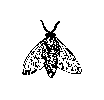
\epsfig{file=fly.eps}
% \caption{A sample black and white graphic (.eps format).}
% \end{figure}

% \begin{figure}
% \centering
% 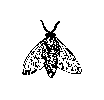
\epsfig{file=fly.eps, height=1in, width=1in}
% \caption{A sample black and white graphic (.eps format)
% that has been resized with the \texttt{epsfig} command.}
% \end{figure}


% As was the case with tables, you may want a figure
% that spans two columns.  To do this, and still to
% ensure proper ``floating'' placement of tables, use the environment
% \textbf{figure*} to enclose the figure and its caption.
% \begin{figure*}
% \centering
% 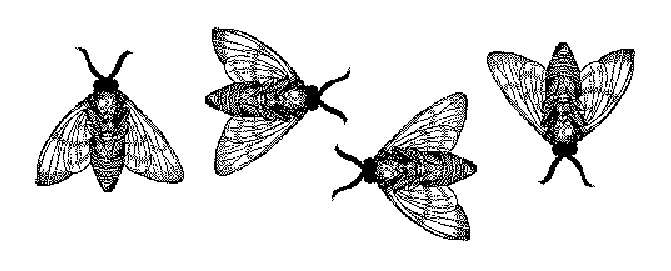
\epsfig{file=flies.eps}
% \caption{A sample black and white graphic (.eps format)
% that needs to span two columns of text.}
% \end{figure*}
% and don't forget to end the environment with
% {figure*}, not {figure}!

% Note that either {\textbf{.ps}} or {\textbf{.eps}} formats are
% used; use
% the \texttt{{\char'134}epsfig} or \texttt{{\char'134}psfig}
% commands as appropriate for the different file types.

% \begin{figure}
% \centering
% \psfig{file=rosette.ps, height=1in, width=1in,}
% \caption{A sample black and white graphic (.ps format) that has
% been resized with the \texttt{psfig} command.}
% \end{figure}

% \subsection{Theorem-like Constructs}
% Other common constructs that may occur in your article are
% the forms for logical constructs like theorems, axioms,
% corollaries and proofs.  There are
% two forms, one produced by the
% command \texttt{{\char'134}newtheorem} and the
% other by the command \texttt{{\char'134}newdef}; perhaps
% the clearest and easiest way to distinguish them is
% to compare the two in the output of this sample document:

% This uses the \textbf{theorem} environment, created by
% the \texttt{{\char'134}newtheorem} command:
% \newtheorem{theorem}{Theorem}
% \begin{theorem}
% Let $f$ be continuous on $[a,b]$.  If $G$ is
% an antiderivative for $f$ on $[a,b]$, then
% \begin{displaymath}\int^b_af(t)dt = G(b) - G(a).\end{displaymath}
% \end{theorem}

% The other uses the \textbf{definition} environment, created
% by the \texttt{{\char'134}newdef} command:
% \newdef{definition}{Definition}
% \begin{definition}
% If $z$ is irrational, then by $e^z$ we mean the
% unique number which has
% logarithm $z$: \begin{displaymath}{\log e^z = z}\end{displaymath}
% \end{definition}

% Two lists of constructs that use one of these
% forms is given in the
% \textit{Author's  Guidelines}.

% There is one other similar construct environment, which is
% already set up
% for you; i.e. you must \textit{not} use
% a \texttt{{\char'134}newdef} command to
% create it: the \textbf{proof} environment.  Here
% is a example of its use:
% \begin{proof}
% Suppose on the contrary there exists a real number $L$ such that
% \begin{displaymath}
% \lim_{x\rightarrow\infty} \frac{f(x)}{g(x)} = L.
% \end{displaymath}
% Then
% \begin{displaymath}
% l=\lim_{x\rightarrow c} f(x)
% = \lim_{x\rightarrow c}
% \left[ g{x} \cdot \frac{f(x)}{g(x)} \right ]
% = \lim_{x\rightarrow c} g(x) \cdot \lim_{x\rightarrow c}
% \frac{f(x)}{g(x)} = 0\cdot L = 0,
% \end{displaymath}
% which contradicts our assumption that $l\neq 0$.
% \end{proof}

% Complete rules about using these environments and using the
% two different creation commands are in the
% \textit{Author's Guide}; please consult it for more
% detailed instructions.  If you need to use another construct,
% not listed therein, which you want to have the same
% formatting as the Theorem
% or the Definition\cite{salas:calculus} shown above,
% use the \texttt{{\char'134}newtheorem} or the
% \texttt{{\char'134}newdef} command,
% respectively, to create it.

% \subsection*{A {\secit Caveat} for the \TeX\ Expert}
% Because you have just been given permission to
% use the \texttt{{\char'134}newdef} command to create a
% new form, you might think you can
% use \TeX's \texttt{{\char'134}def} to create a
% new command: \textit{Please refrain from doing this!}
% Remember that your \LaTeX\ source code is primarily intended
% to create camera-ready copy, but may be converted
% to other forms -- e.g. HTML. If you inadvertently omit
% some or all of the \texttt{{\char'134}def}s recompilation will
% be, to say the least, problematic.

% \section{Conclusions}
% This paragraph will end the body of this sample document.
% Remember that you might still have Acknowledgments or
% Appendices; brief samples of these
% follow.  There is still the Bibliography to deal with; and
% we will make a disclaimer about that here: with the exception
% of the reference to the \LaTeX\ book, the citations in
% this paper are to articles which have nothing to
% do with the present subject and are used as
% examples only.
% %\end{document}  % This is where a 'short' article might terminate

% %ACKNOWLEDGMENTS are optional
% \section{Acknowledgments}
% This section is optional; it is a location for you
% to acknowledge grants, funding, editing assistance and
% what have you.  In the present case, for example, the
% authors would like to thank Gerald Murray of ACM for
% his help in codifying this \textit{Author's Guide}
% and the \textbf{.cls} and \textbf{.tex} files that it describes.

% %
% The following two commands are all you need in the
% initial runs of your .tex file to
% produce the bibliography for the citations in your paper.
\bibliographystyle{abbrv}
\bibliography{report}  % sigproc-sp-csis8101.bib is the name of the Bibliography in this case
% You must have a proper ".bib" file
%  and remember to run:
% latex bibtex latex latex
% to resolve all references
%
% ACM needs 'a single self-contained file'!
%
%APPENDICES are optional
%\balancecolumns
% \appendix
% %Appendix A
% \section{Headings in Appendices}
% The rules about hierarchical headings discussed above for
% the body of the article are different in the appendices.
% In the \textbf{appendix} environment, the command
% \textbf{section} is used to
% indicate the start of each Appendix, with alphabetic order
% designation (i.e. the first is A, the second B, etc.) and
% a title (if you include one).  So, if you need
% hierarchical structure
% \textit{within} an Appendix, start with \textbf{subsection} as the
% highest level. Here is an outline of the body of this
% document in Appendix-appropriate form:
% \subsection{Introduction}
% \subsection{The Body of the Paper}
% \subsubsection{Type Changes and  Special Characters}
% \subsubsection{Math Equations}
% \paragraph{Inline (In-text) Equations}
% \paragraph{Display Equations}
% \subsubsection{Citations}
% \subsubsection{Tables}
% \subsubsection{Figures}
% \subsubsection{Theorem-like Constructs}
% \subsubsection*{A Caveat for the \TeX\ Expert}
% \subsection{Conclusions}
% \subsection{Acknowledgments}
% \subsection{Additional Authors}
% This section is inserted by \LaTeX; you do not insert it.
% You just add the names and information in the
% \texttt{{\char'134}additionalauthors} command at the start
% of the document.
% \subsection{References}
% Generated by bibtex from your ~.bib file.  Run latex,
% then bibtex, then latex twice (to resolve references)
% to create the ~.bbl file.  Insert that ~.bbl file into
% the .tex source file and comment out
% the command \texttt{{\char'134}thebibliography}.
% % This next section command marks the start of
% % Appendix B, and does not continue the present hierarchy
% \section{More Help for the Hardy}
% The acm\_proc\_article-sp document class file itself is chock-full of succinct
% and helpful comments.  If you consider yourself a moderately
% experienced to expert user of \LaTeX, you may find reading
% it useful but please remember not to change it.



% That's all folks!
\end{document}
